\documentclass[10pt,a4paper]{article}
\usepackage[utf8]{inputenc}
\usepackage{amsmath}
\usepackage{amsfonts}
\usepackage{amssymb}
\usepackage{graphicx}
\author{Andrea Colarieti Tosti}
\title{Rechenarchitektur Tutorium 4 Lösung}

\begin{document}
\maketitle

\section{Aufgabe 20}
\subsection{A}
KNF($f$) = 
\begin{equation*}
( x_{1} + x_{2}  + x_{2} + \overline{x_{4}} )* 
( x_{1} + \overline{x_{2} } + \overline{x_{3}} + x_{4} )*
( x_{1} + \overline{x_{2} } + \overline{x_{3}} + \overline{x_{4}} )*
( \overline{x_{1} } + x_{2} + x_{3} + x_{4} )*
(  \overline{x_{1} } + x_{2} + \overline{x_{3}} + \overline{x_{4}} )*
( \overline{x_{1} } + \overline{x_{2} } + \overline{x_{3}} + x_{4} )
\end{equation*}

\subsection{B}
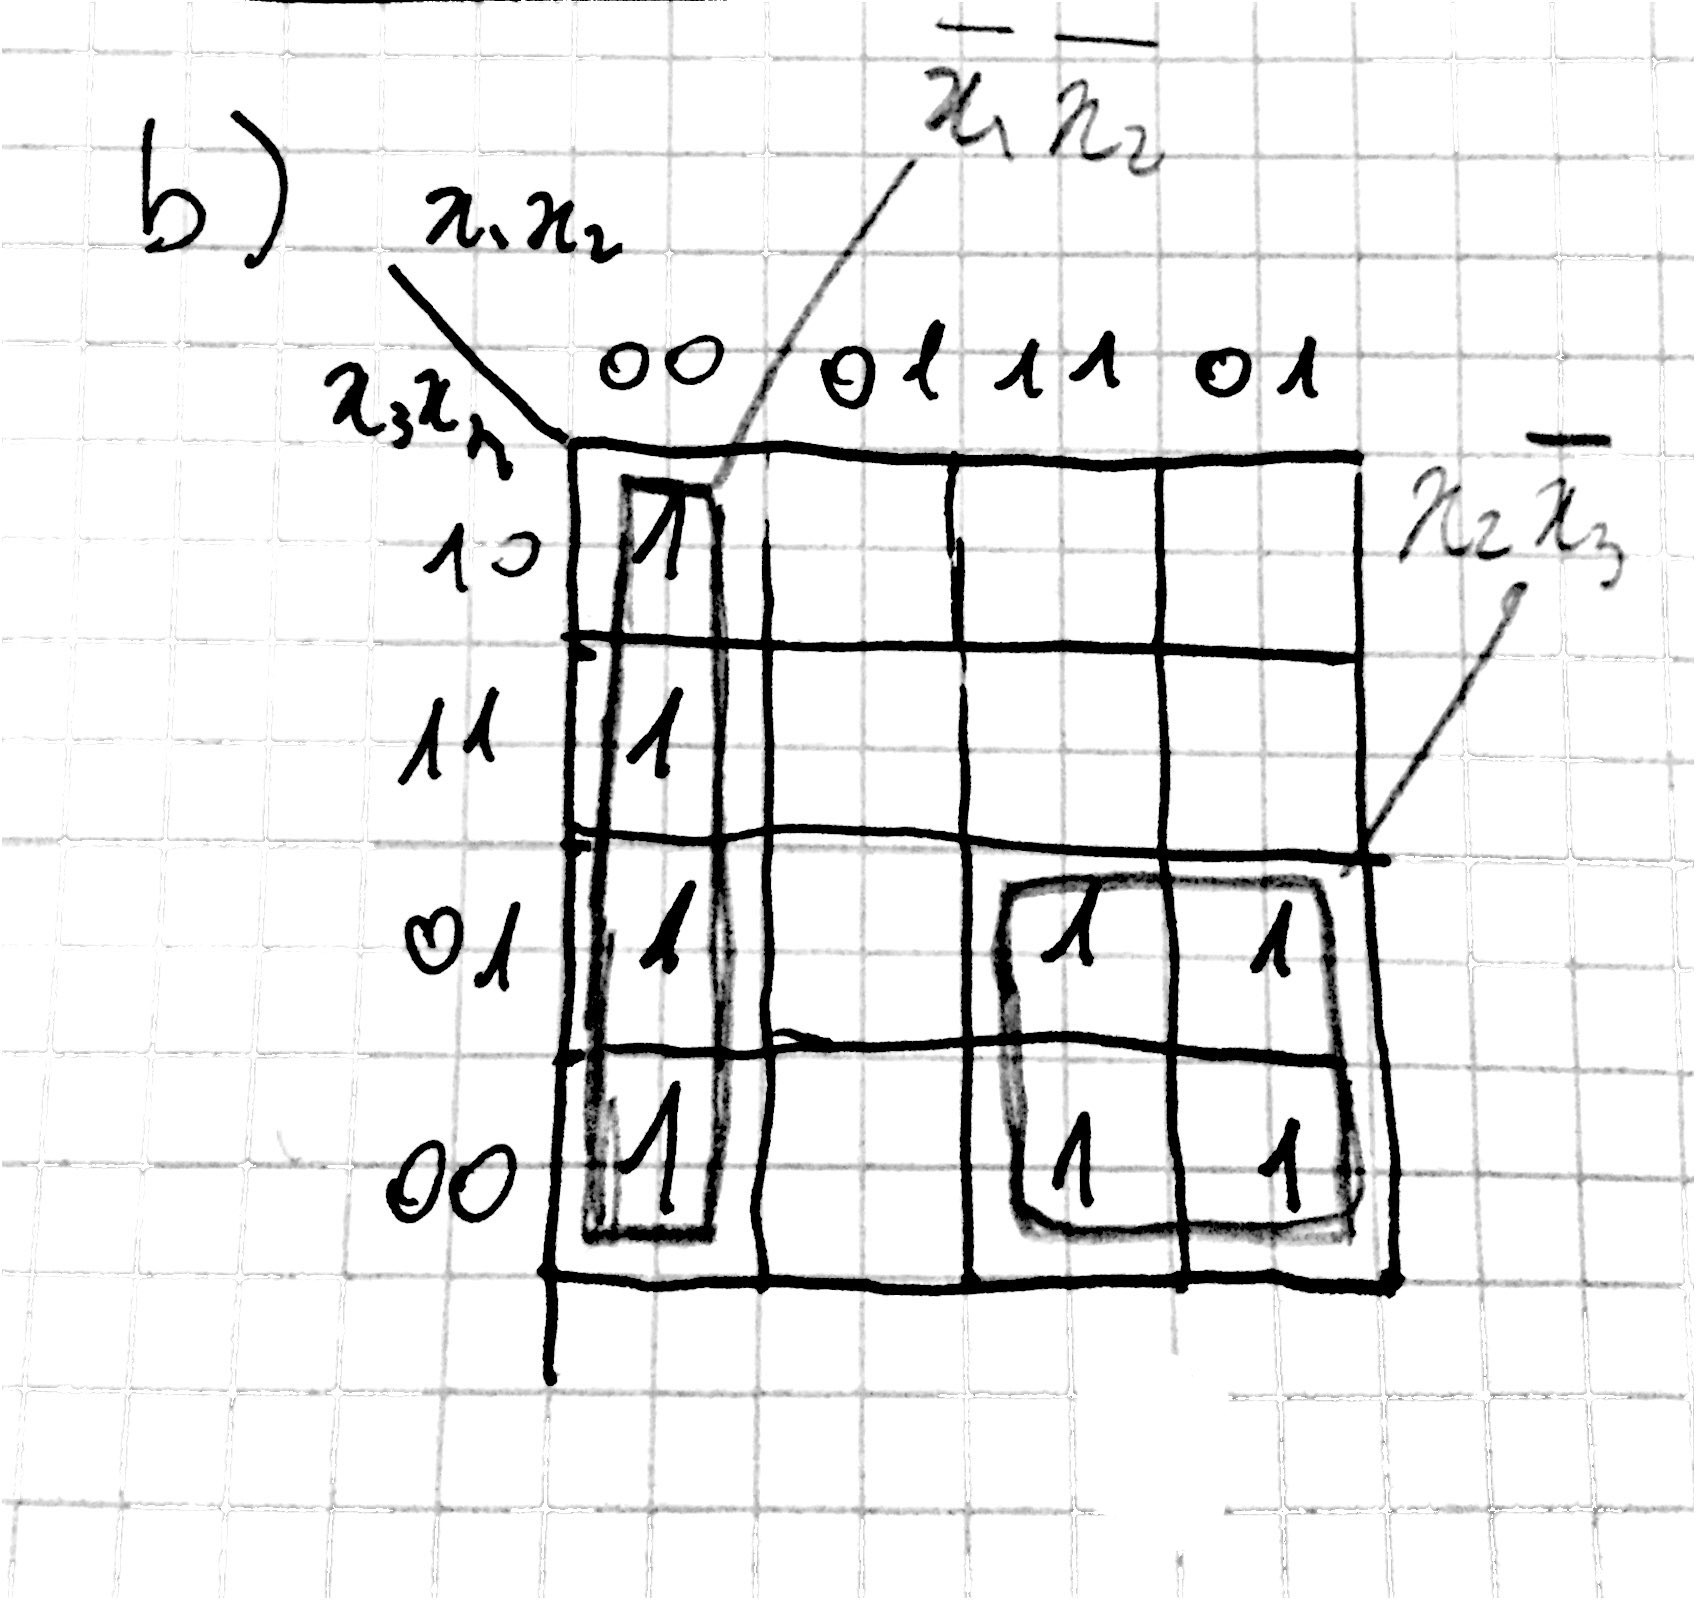
\includegraphics[scale=0.2]{RA_t4_1.jpg} \newline
DNF($g$) =  $ (x_{1}\overline{x_{3}})+(\overline{x_{1}} \overline{x_{2}})$

\section{Aufgabe 21}

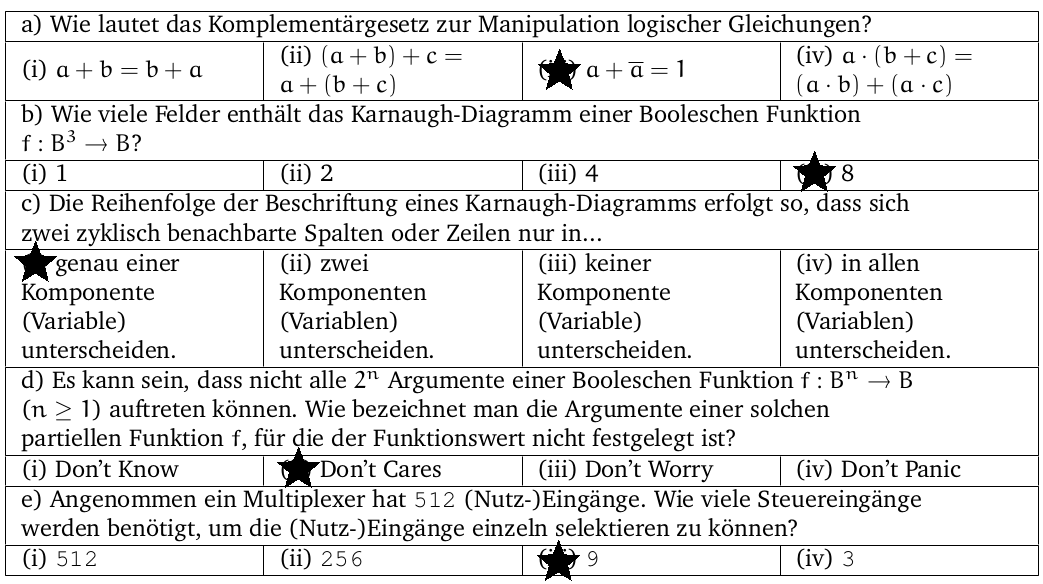
\includegraphics[scale=0.35]{MultiChoice.png} 

\end{document} 